\chapter{Results}
\textit{In this chapter the results from the data analysis will be shown. Box plots and a table will present the mean magnitude values. A paired t-test is was used to test the likelihood of finding a difference between the baseline and restricted condition.}

The box plots can be seen in \figref{fig:boxEndo} throughout \figref{fig:boxMyo}. The box plots show points for each mean magnitude for each subject ordered by color, a line is connecting the before and after condition to indicate if there has been an increase or decrease in magnitude. 

\begin{figure}[H]
	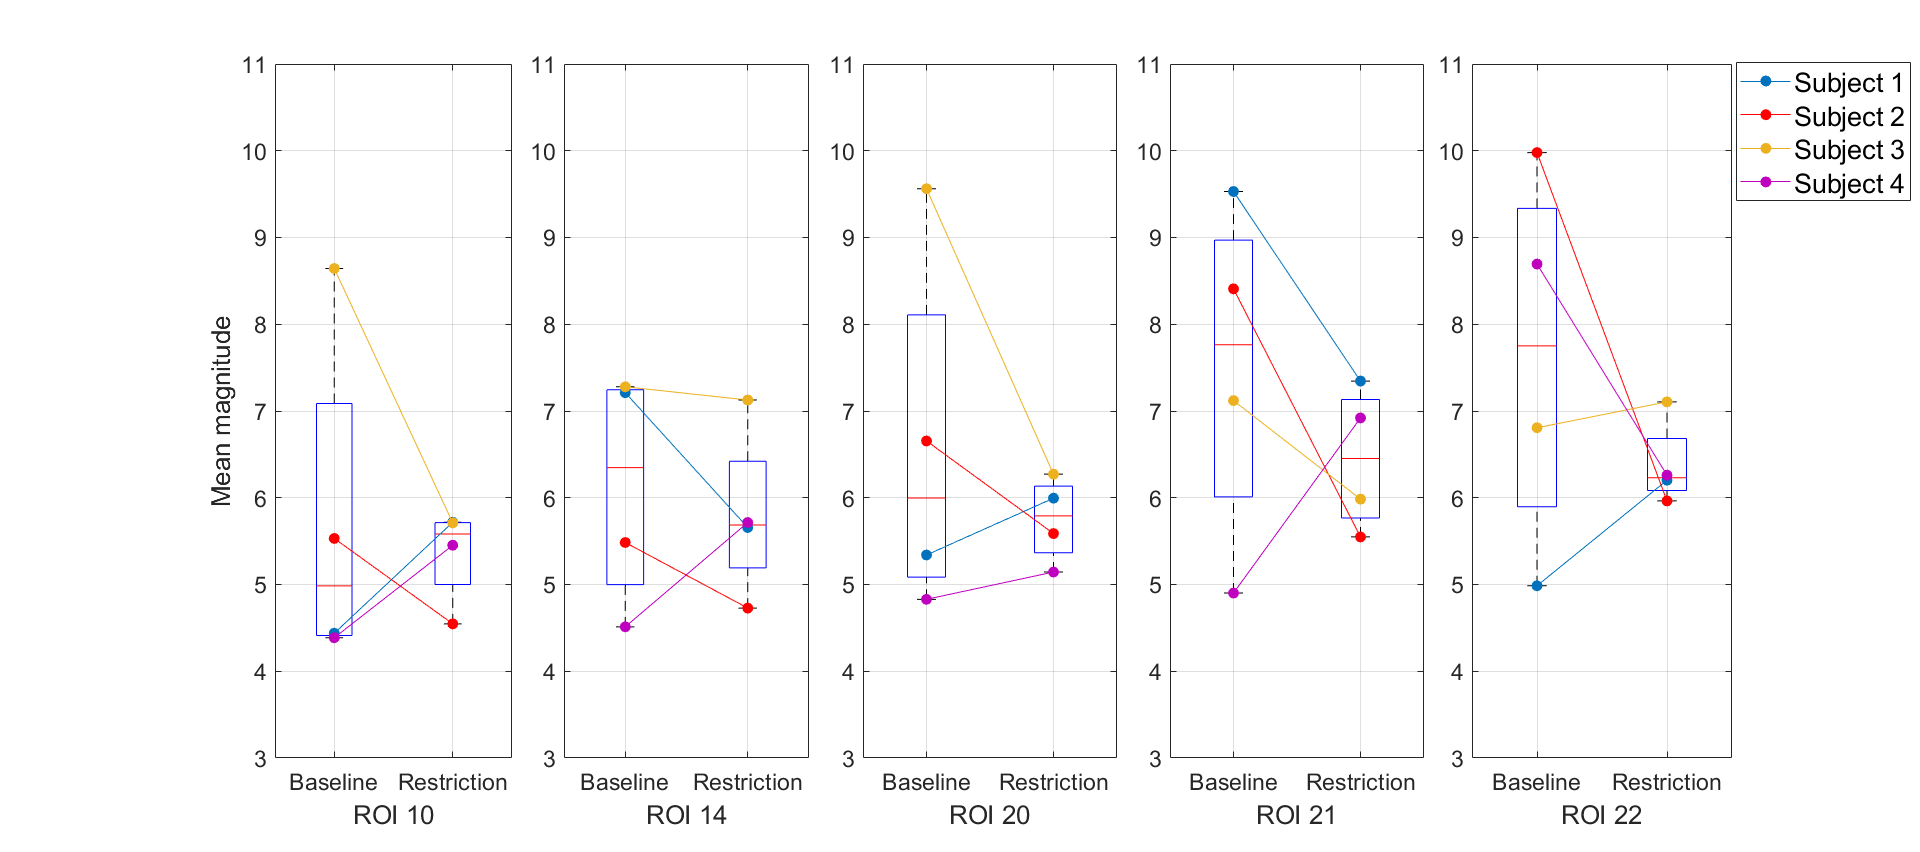
\includegraphics[width=1\textwidth]{figures/boxplot_endo}
	\caption{Box plot for mean magnitude in the endothelial frequency band, for both conditions in five ROIs.}
	\label{fig:boxEndo}
\end{figure}

\begin{figure}[H]
	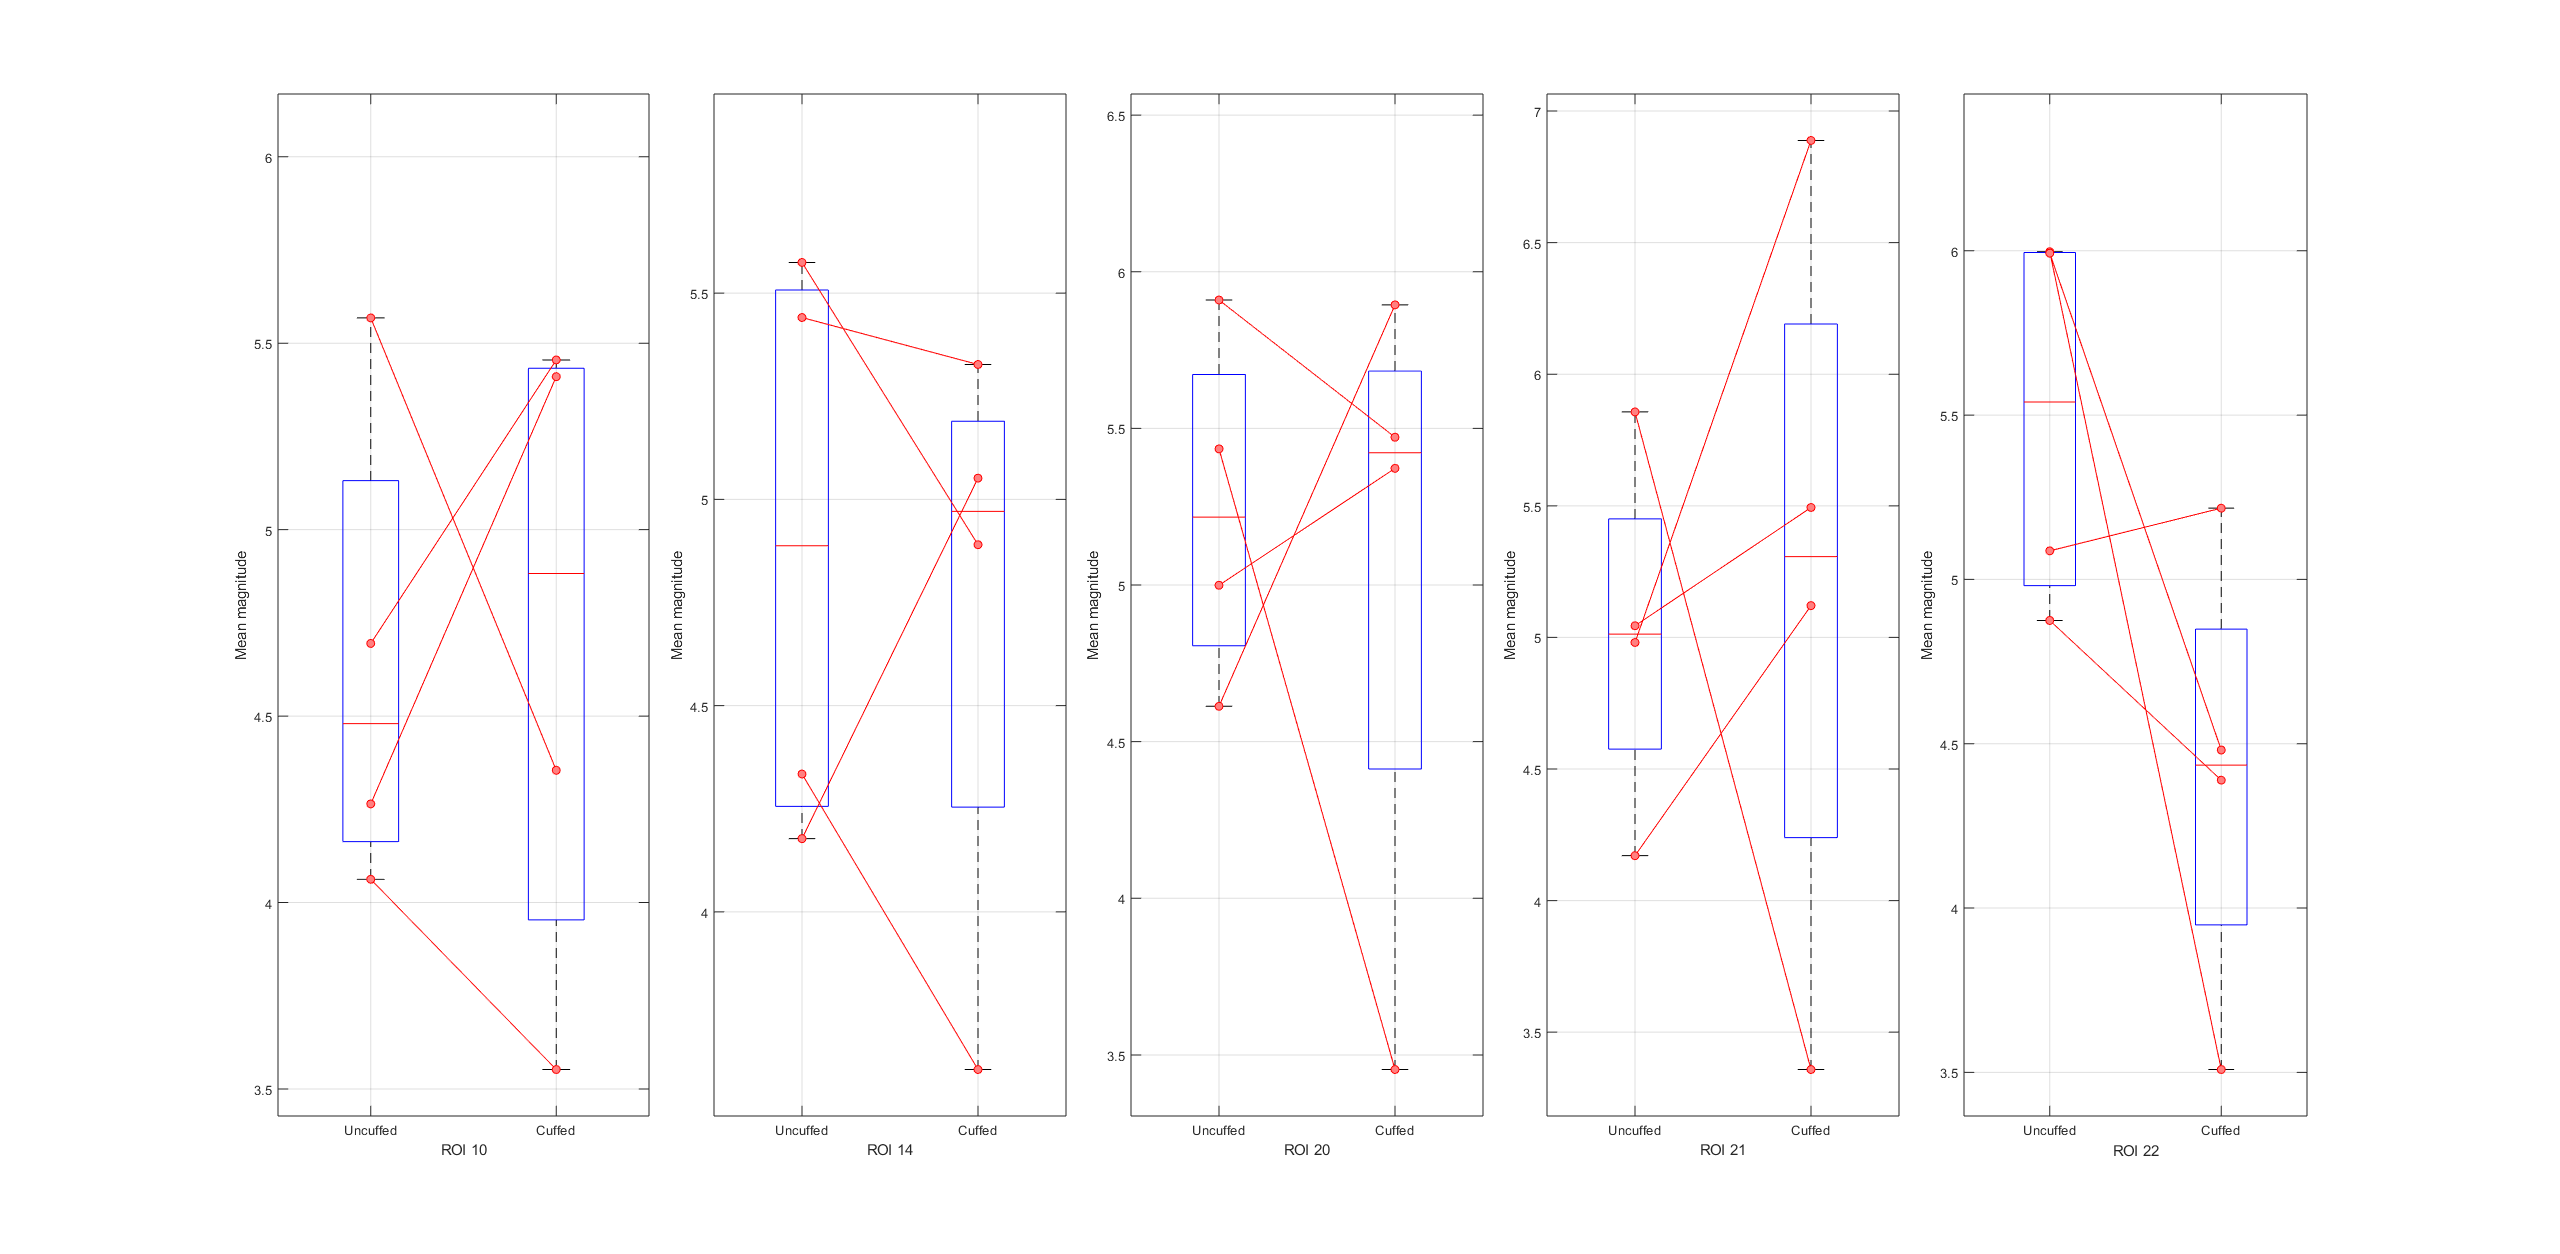
\includegraphics[width=1\textwidth]{figures/boxplot_neuro}
	\caption{Box plot for mean magnitude in the neurogenic frequency band, for both conditions in five ROIs.}
	\label{fig:boxNeuro}
\end{figure}

\begin{figure}[H]
	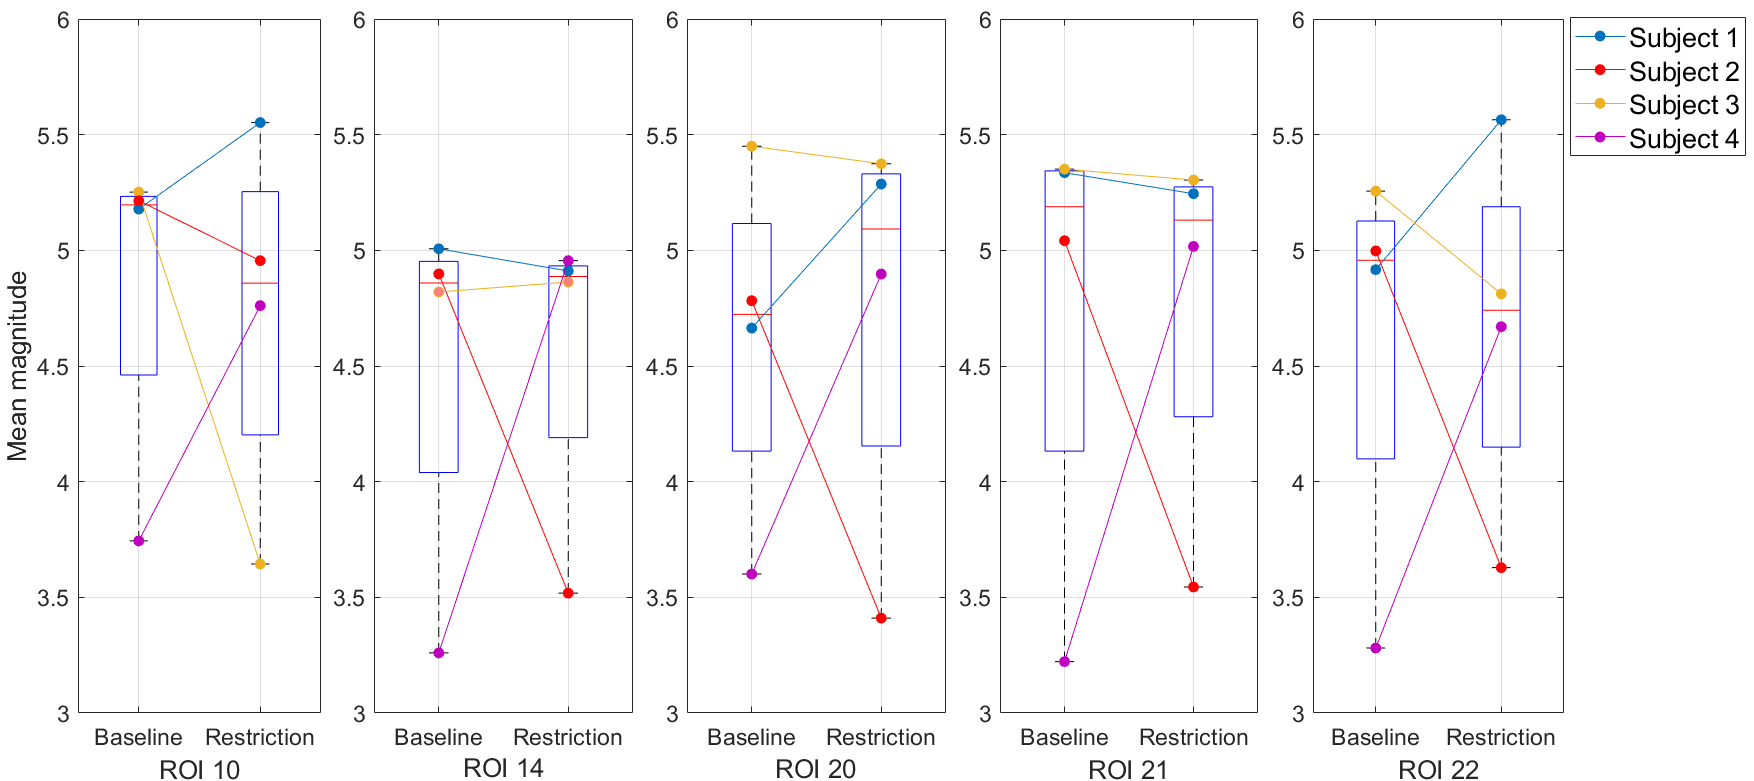
\includegraphics[width=1\textwidth]{figures/boxplot_myo}
	\caption{Box plot for mean magnitude in the myogenic frequency band, for for both conditions in five ROIs.}
	\label{fig:boxMyo}
\end{figure}
 
 Table \ref{my:mean} illustrates a mean magnitude value for endothelial, neurogenic and myogenic frequency band in the baseline and restricted measurement. The mean magnitude values are representing all subjects and ROIs. 
 \begin{table} [thpb]
 	\caption{Table showing the mean magnitudes of each frequency band in both measured conditions.}
 	\label{my:mean}
 	\centering
 	\scalebox{0.8}{
 		\begin{tabular}{l|lll}
 			
 			& \textbf{mean endo} & \textbf{mean neuro}  & \textbf{mean myo} \\ \hline
 			\textbf{Baseline} & 6.71$\pm$1.90 & 5.05$\pm$0.65 & 4.66$\pm$0.77   \\ \hline
 			\textbf{Restriction} & 5.95$\pm$0.75 & 4.82$\pm$0.95 &  4.70$\pm$0.72  \\ \hline
 	\end{tabular}}
 	
 \end{table}

%In the paired t-test none of the data from the frequency bands show a significant difference between subject in cuffed and uncuffed condition. 
The outcome of the paired t-test is a table showing the p-values, which is shown in \cref{my:pval}. 
\begin{table}[H]
	\centering
	\caption{Table showing the p-values corresponding to specific ROI in correlation with frequency band.}
	\scalebox{0.8}{
	\begin{tabular}{l|lll}
		
		& \textbf{p-endo} & \textbf{p-neuro}  & \textbf{p-myo} \\ \hline
		\textbf{ROI 10} & 0.71 & 0.93 & 0.84  \\ \hline
		\textbf{ROI 14} & 0.62 & 0.69 & 0.92  \\ \hline
		\textbf{ROI 20} & 0.41 & 0.80 & 0.84  \\ \hline
		\textbf{ROI 21} & 0.40 & 0.84 & 0.95  \\ \hline
		\textbf{ROI 22} & 0.38 & 0.15 & 0.93  \\ \hline
	\end{tabular}}
	\label{my:pval}
\end{table}
As indicated in table \ref{my:pval}, all of the tests show a significance level well above 0.05, which means that $h_{0}$ is not rejected, whereby there is no significant difference between the two conditions. %The lowest p-value is presented in region 22 where a p-value of 0.1552 for the neurogenic band is found. 
%When reflecting the p-values onto the box plots the correlation between the p-values and the occurrence of a difference in the dataset can be seen. For instance the lowest p-value of 0.1552 indicates the greatest difference between means, this can also be seen in \figref{fig:boxNeuro} for ROI 22. 
  
%\section{T-value mapping}
%Results illustrated on \figref{fig:black}, shows a t-value mapped image from a summation of each subjects scalogram within the two conditions. The y-axis shows the number of different frequencies and the x-axis is time, giving in number of frames. Each pixel within the image has a t-value corresponding to the test of the uncuffed pixel value compared to the cuffed pixel value. The larger t-value, the brighter a pixel will appear in the image. The image showed no areas where a greater difference could be observed. Mostly individual pixels lid up showing a great difference, but as these are individual and not part of an area, these are considered outliers.  

%\begin{figure}[H]
%	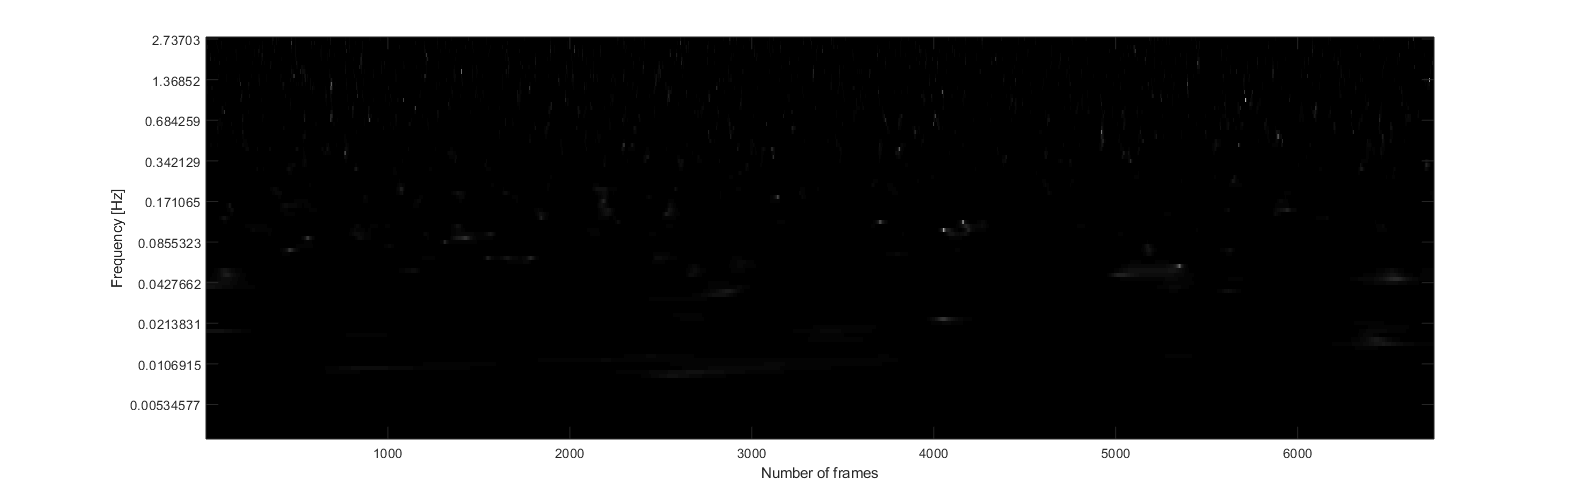
\includegraphics[width=1\textwidth]{figures/t-values_roi10}
%	\caption{t-value mapped image, from a t-test of region 10, uncuffed versus cuffed.}
%	\label{fig:black}
%\end{figure}

%Neither of the images corresponding to each region showed areas where vasomotion activity could be identified. The remaining t-value mapping images can be seen in \cref{t-value}.  
%The number of positive and negative t-values for each frequency band in every region is compared in \cref{tab:t}. Positive t-values indicate a drop in amplitude from the uncuffed state to the cuffed and negative values the opposite. No  
%\begin{table}[H]
%	\centering
%	\caption{Table with comparison of t-values for every band at every region.}
%	\label{tab:t}
%	\scalebox{0.7}{
%	\begin{tabular}{|l|l|l|l|}
%		\hline
%		& Endo band      & Neuro band     & Myo band       \\ \hline
%		\multicolumn{4}{|l|}{Region 10}                                         \\ \hline
%		Positive vs negative & 76377 vs 65352 & 49665 vs 38072 & 55092 vs 52892 \\ \hline
%		\multicolumn{4}{|l|}{Region 20}                                         \\ \hline
%		Positive vs negative & 79309 vs 62428 & 44248 vs 43489 & 52116 vs 55968 \\ \hline
%		\multicolumn{4}{|l|}{Region 21}                                         \\ \hline
%		Positive vs negative & 74634 vs 67095 & 43542 vs 44195 & 52941 vs 55043 \\ \hline
%		\multicolumn{4}{|l|}{Region 22}                                         \\ \hline
%		Positive vs negative & 88601 vs 53128 & 64195 vs 23542 & 51462 vs 56522 \\ \hline
%	\end{tabular}}
%\end{table}
%T is simply the calculated difference represented in units of standard error. The greater the magnitude of T (it can be either positive or negative), the greater the evidence against the null hypothesis that there is no significant difference. The closer T is to 0, the more likely there isn't a significant difference.

%\section{ANOVA}